\begin{event}{Sage Days 98 : Women in Sage}{SD98}{Archanes (Greece), April 8 -- April 12, 2019}{PS}{22}{1}{https://opendreamkit.org/2019/06/28/WomenInSage/}

\textbf{Main goals.} The main goal of the event was to initiate more women to the software \Sage to reduce the gender gap in mathematics software
development. Each participant had to propose a mathematic development project to be carried out during the week.

\textbf{\ODK implication.} The event was initiated by Viviane Pons from \ODK and co-organized with Eleni Tzanaki (University of Crete). It was funded solely by \ODK which covered: lodging for the participants (rented houses), food, and transportation for many of the participants.

\textbf{Event summary.} The event was organized as a workshop where every participant could work on their own project to develop their coding skills. We started the week with an introduction to Sage and some tutorials. Then each participant gave a 5 minute talk about their own research. After that, we worked on different projects, organizing status reports every day. In particular, we ran a group specifically to produce new contributions to Sage.

\textbf{Demographics.} All participants were women coming from 8 different countries (France, Belgium, Germany, Greece, UK, US, Romania and Peru), as per institutions, and more if we count nationalities (Australia, Lebanon, Spain). About half of them could be considered Sage beginners. We had 1 master student, 14 PhD students, 2 postdocs, and 5 \textit{Maîtresses de conférences} or assistant professor or lecturer.

We were supposed to also welcome 3 women from Nigeria but they were sadly not able to obtain their visas on time.

\textbf{Results and impact.} A full report on the impact of this
workshop can be read on our website:
\centerline{\url{https://opendreamkit.org/2019/06/28/WomenInSage/}}
The main goal was to make the participants more confident into their programming skills and more prone to become Sage contributors and attend classical Sage Days. It was a big success in that regard. Indeed, before the conference, only 17\% of the participants had attended Sage Days more than once and 50\% had never heard of it. After, the conference, 94\% rated 3 or more out of 5 the chances that they would attend Sage Days event in the future. 100\% of the participant rated 3 or more out of 5 the impact of the workshop on their future career and 100\% said they met interesting people. Additionally, work was done on 5 Sage issues from of which 3 have been merged into Sage source code already.

\begin{figure}[ht]
  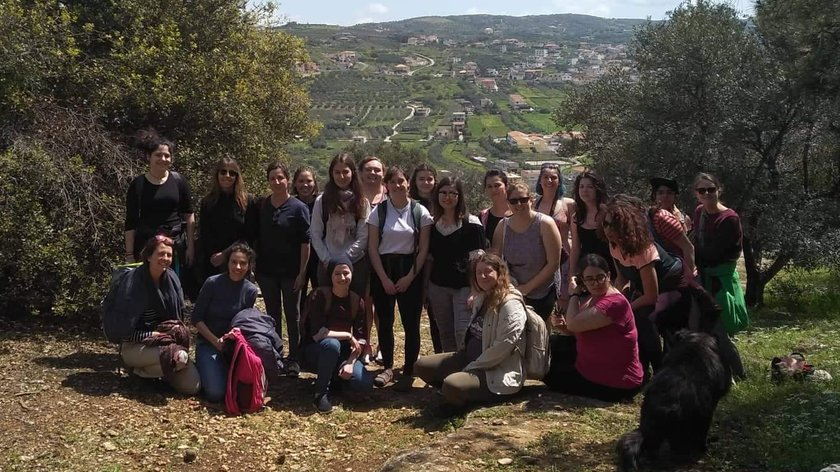
\includegraphics[width=.75\textwidth]{group_photo_head.jpeg}
  \caption*{Women in Sage, Archanes, Crete}
\end{figure}



\end{event}
